\documentclass[11pt,a4paper]{article}

% ---------- Packages ----------
\usepackage[margin=2.2cm]{geometry}
\usepackage{graphicx}
\usepackage{booktabs}
\usepackage{amsmath}
\usepackage{float}
\usepackage{caption}
\usepackage{subcaption}
\usepackage{hyperref}
\usepackage{xcolor}
\usepackage{array}

\hypersetup{
  colorlinks=true,
  linkcolor=blue!50!black,
  urlcolor=blue!50!black,
  citecolor=blue!50!black
}

\captionsetup{font=small,labelfont=bf}



\section{Introduction}

The dataset used is the primary training sample released by the NYC
Taxi and Limousine Commission (TLC) for the Kaggle \emph{NYC Taxi Trip
Duration} competition. It contains 1{,}458{,}644 trips between
2016-01-01 and 2016-06-30 with 11 columns: \texttt{id},
\texttt{vendor\_id}, \texttt{pickup\_datetime}, \texttt{dropoff\_datetime},
\texttt{passenger\_count}, \texttt{pickup\_longitude},
\texttt{pickup\_latitude}, \texttt{dropoff\_longitude},
\texttt{dropoff\_latitude}, \texttt{store\_and\_fwd\_flag} and
\texttt{trip\_duration} (seconds). No distance or speed column is
provided, and both must be derived. All analyses below are performed on
the \emph{cleaned} frame unless otherwise stated.


\section{Data Cleaning}

\subsection{Initial diagnostics}

\begin{table}[H]
\centering
\caption{Summary statistics of the raw (uncleaned) frame.
\texttt{distance\_km} is haversine great-circle distance between pickup
and dropoff.}
\label{tab:raw-summary}
\begin{tabular}{lrrr}
\toprule
 & \texttt{trip\_duration} (s) & \texttt{distance\_km} & \texttt{speed\_kmh} \\
\midrule
count & 1{,}458{,}644 & 1{,}458{,}644 & 1{,}458{,}644 \\
mean  & 959.49        & 3.44          & 14.41 \\
std   & 5{,}237.43    & 4.29          & 14.97 \\
min   & 1.00          & 0.00          & 0.00 \\
1\,\%  & 87.00         & 0.14          & 1.39 \\
50\,\% & 662.00        & 2.09          & 12.78 \\
99\,\% & 3{,}440.00    & 20.77         & 40.72 \\
max   & 3{,}526{,}282 & 1{,}240.13    & 9{,}269.01 \\
\bottomrule
\end{tabular}
\end{table}

The maximum trip duration is \textbf{40.8 days}, the maximum haversine
distance is \textbf{1{,}240\,km} (roughly the distance to Chicago) and
the maximum implied speed is \textbf{9{,}269\,km/h}. None of these are
physically possible taxi trips inside New York City. Further
row-level diagnostics yield:

\begin{itemize}
  \item \texttt{trip\_duration} $\le 0$: 0 rows (minimum is 1\,s);
  \item \texttt{trip\_duration} $> 6$\,h: 2{,}061 rows;
  \item zero-distance trips: 5{,}897 rows;
  \item \texttt{speed\_kmh} $> 100$: 175 rows;
  \item \texttt{speed\_kmh} $< 1$: 13{,}241 rows;
  \item pickup outside the NYC bounding box: 256 rows;
  \item \texttt{passenger\_count}: 60 trips with 0, and 5 trips with
        counts of 7, 8 or 9 (above the legal capacity of a standard cab).
\end{itemize}

\newpage

\subsection{Cleaning rules and justification}
Each filter is motivated by a physical or operational argument:

\begin{table}[H]
\centering
\caption{Cleaning rules applied and their justification.}

\begin{tabular}{p{3.4cm}p{4.3cm}p{7.4cm}}
\toprule
\textbf{Rule} & \textbf{Threshold} & \textbf{Justification} \\
\midrule
Duration lower bound & $\texttt{trip\_duration} \ge 30$\,s &
  Sub-30\,s trips are meter toggles, cancellations or GPS clock errors;
  they carry no travel information. \\
Duration upper bound & $\texttt{trip\_duration} \le 6$\,h &
  NYC is $\approx 60$\,km across; even the longest realistic airport
  round-trips do not exceed a few hours. Multi-day values are
  ``meter-left-running'' records. \\
Speed bounds & $1 \le \texttt{speed\_kmh} \le 100$ &
  The 1\,km/h floor removes stationary GPS records (waiting, signal
  loss). The 100\,km/h ceiling is above any legal city speed limit and
  above any attainable \emph{average} speed on NYC roads. \\
Geographic box & lat $\in [40.5, 41.0]$, lon $\in [-74.3, -73.7]$ &
  Covers all five boroughs plus JFK, LGA and EWR. Points outside are
  GPS glitches (e.g.\ $(0,0)$) or fat-finger entries. \\
Non-zero distance & $\texttt{distance\_km} > 0$ &
  A zero-distance trip with non-zero duration is a meter movement or
  GPS failure and has no spatial content. \\
Passenger count & $1 \le \texttt{passenger\_count} \le 6$ &
  \texttt{0} is a data-entry error; $>6$ exceeds legal cab capacity. \\
\bottomrule
\end{tabular}
\end{table}

\subsection{Retention and effect}
Table 3 reports the retention of each filter applied
independently.The intersection of all five filters retains
\textbf{1{,}442{,}031 rows (98.86\,\%)}.

\begin{table}[H]
\centering
\caption{Individual filter retention.}

\begin{tabular}{lrr}
\toprule
\textbf{Filter} & \textbf{Rows kept} & \textbf{Share} \\
\midrule
Duration 30\,s -- 6\,h        & 1{,}451{,}801 & 99.53\,\% \\
Speed 1 -- 100\,km/h          & 1{,}445{,}228 & 99.08\,\% \\
Coordinates in NYC bbox       & 1{,}457{,}646 & 99.93\,\% \\
Distance $> 0$                & 1{,}452{,}747 & 99.60\,\% \\
Passenger count 1--6          & 1{,}458{,}579 & 100.00\,\% \\
\midrule
\textbf{All filters (joint)}  & \textbf{1{,}442{,}031} & \textbf{98.86\,\%} \\
\bottomrule
\end{tabular}
\end{table}


\newpage
The cleaned distribution is now bounded
and realistic: median duration 664\,s (11.1\,min), median haversine
distance 2.11\,km, median speed 12.85\,km/h, and the standard deviation
of duration collapses from 5{,}237\,s to 656\,s. Removing the outliers is
justified because they are \emph{not a random sample} of the data---they
are concentrated in the tails---so every mean, plot and model downstream
would be biased by them; and because they are demonstrably not real taxi
trips, they carry no useful signal about travel demand.

\begin{table}[H]
\centering
\caption{Cleaned summary statistics.}

\begin{tabular}{lrrr}
\toprule
 & \texttt{trip\_duration} (s) & \texttt{distance\_km} & \texttt{speed\_kmh} \\
\midrule
count & 1{,}442{,}031 & 1{,}442{,}031 & 1{,}442{,}031 \\
mean  & 838.80        & 3.45          & 14.48 \\
std   & 656.25        & 3.88          & 7.62 \\
min   & 30.00         & 0.009         & 1.00 \\
25\,\% & 400.00        & 1.251         & 9.22 \\
50\,\% & 664.00        & 2.112         & 12.85 \\
75\,\% & 1{,}074.00    & 3.896         & 17.88 \\
max   & 21{,}411.00   & 47.735        & 99.47 \\
\bottomrule
\end{tabular}
\end{table}


\section{Feature Generation}
 The
\texttt{distance\_km} and \texttt{speed\_kmh} features are generated
\emph{before} cleaning so that the speed filter can be applied to every
row; the time features are generated \emph{after} cleaning.

\begin{table}[H]
\centering
\caption{Generated features.}

\begin{tabular}{p{3.2cm}p{4.6cm}p{7.3cm}}
\toprule
\textbf{Feature} & \textbf{Definition} & \textbf{Purpose} \\
\midrule
\texttt{distance\_km} & Haversine(pickup, dropoff) &
  The dataset ships no distance column; every speed/spatial analysis
  depends on it. Haversine is a straight-line (``as the crow flies'')
  proxy and underestimates road distance by 20--40\,\% in Manhattan,
  but is consistent and computable. \\
\texttt{speed\_kmh} & \texttt{distance\_km} and trip duration &
  Physically interpretable; used for the Q1 filter and Q3.5 analysis. \\
\texttt{pickup\_dow} & \texttt{dt.dayofweek}, Monday$=0$ &
  Integer day-of-week for grouping and plotting. \\
\texttt{day\_name} & \texttt{dt.day\_name()} &
  Human-readable day for tables and plots. \\
\texttt{pickup\_hour} & \texttt{dt.hour} &
  Hourly analysis for Q3.2, Q3.4 and Q3.5. \\
\texttt{is\_weekend} & \texttt{pickup\_dow} $\ge 5$ &
  Boolean split for Q3.3. \\
\bottomrule
\end{tabular}
\end{table}

\newpage


\begin{table}[H]
\centering
\caption{Trip counts by day of week (cleaned frame).}

\begin{tabular}{lrr}
\toprule
\textbf{Day} & \textbf{Trips} & \textbf{Share (\%)} \\
\midrule
Monday    & 185{,}308 & 12.85 \\
Tuesday   & 200{,}459 & 13.90 \\
Wednesday & 207{,}871 & 14.42 \\
Thursday  & 216{,}049 & 14.98 \\
Friday    & 220{,}968 & 15.32 \\
Saturday  & 218{,}393 & 15.15 \\
Sunday    & 192{,}983 & 13.38 \\
\bottomrule
\end{tabular}
\end{table}


\section{Time-Based Analysis}

All times below use \texttt{pickup\_datetime}.

\subsection{Q3.1 --- Most popular day of the week}
\textbf{Answer: Friday, with 220{,}968 trips (15.32\,\%).} The least
popular day is Monday (185{,}308 trips, 12.85\,\%). 

\begin{figure}[H]
\centering
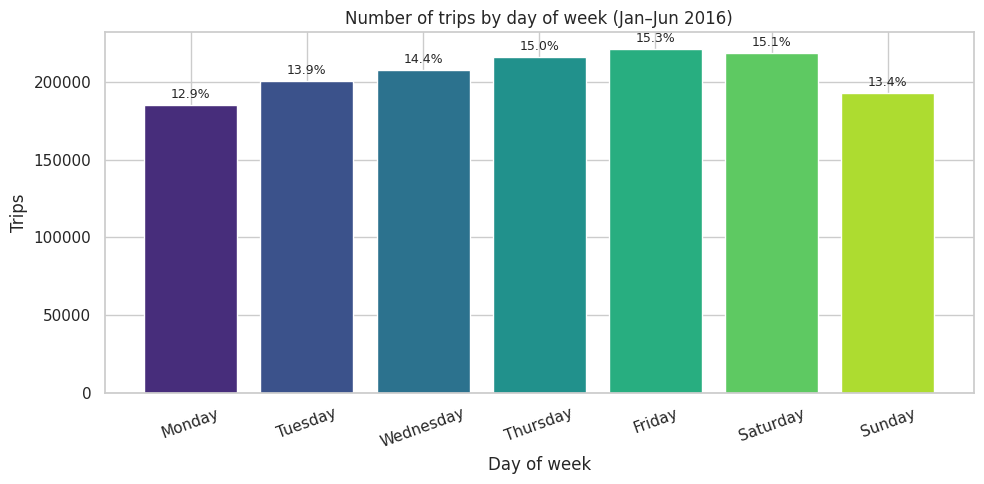
\includegraphics[width=0.82\textwidth]{q3_1_day_of_week.png}
\caption{Trips by day of week with percentage shares. Friday is the
busiest day and Monday the quietest.}

\end{figure}

Demand ramps up steadily from Monday through Friday, plateaus over the
weekend and falls sharply on Sunday. Friday combines the end of the
working week (commuting plus after-work socialising) with the start of
the weekend (nightlife, visitors), while Sunday loses the weekday
commuter and the business traveller. 

\newpage

\subsection{Q3.2 --- Peak hour on each day}
\textbf{Peak hour per day and peak trip counts} are given in
Table 7. Figure 7.a and b shows the day~$\times$~hour
heatmap and the per-day normalised hourly profile.

\begin{table}[H]
\centering
\caption{Peak pickup hour per day and the corresponding peak trip count.}
\begin{tabular}{lrr}
\toprule
\textbf{Day} & \textbf{Peak hour} & \textbf{Peak trips} \\
\midrule
Monday    & 18:00 & 12{,}829 \\
Tuesday   & 18:00 & 13{,}328 \\
Wednesday & 19:00 & 13{,}573 \\
Thursday  & 21:00 & 14{,}019 \\
Friday    & 19:00 & 14{,}030 \\
Saturday  & 23:00 & 13{,}051 \\
Sunday    & 00:00 & 12{,}143 \\
\bottomrule
\end{tabular}
\end{table}

\begin{figure}[H]
\centering
\begin{subfigure}{0.49\textwidth}
  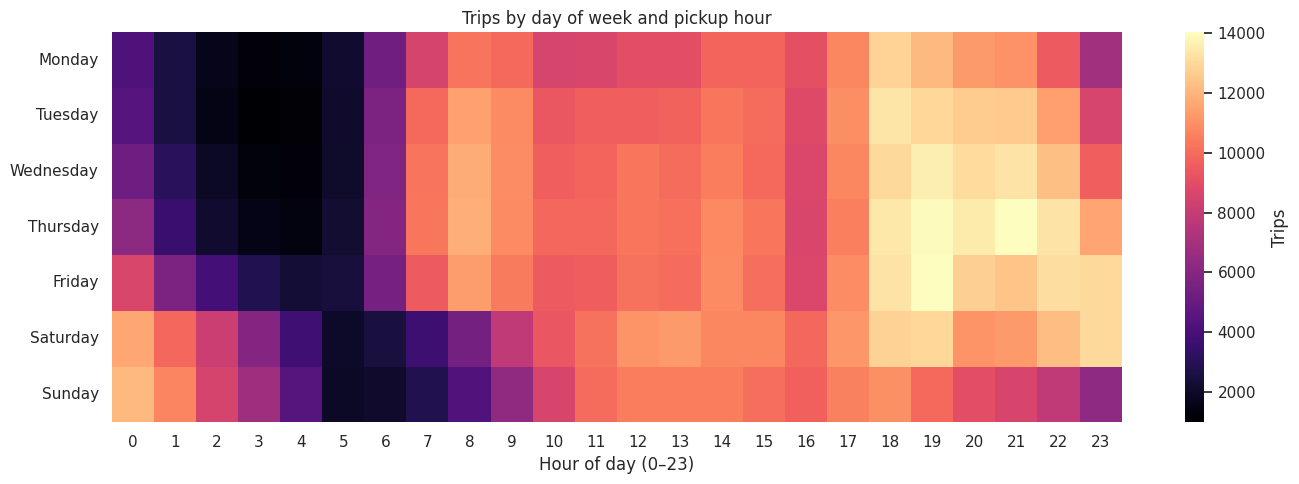
\includegraphics[width=\linewidth]{q3_2_heatmap.png}
  \caption{Day~$\times$~hour heatmap.}
\end{subfigure}\hfill
\begin{subfigure}{0.49\textwidth}
  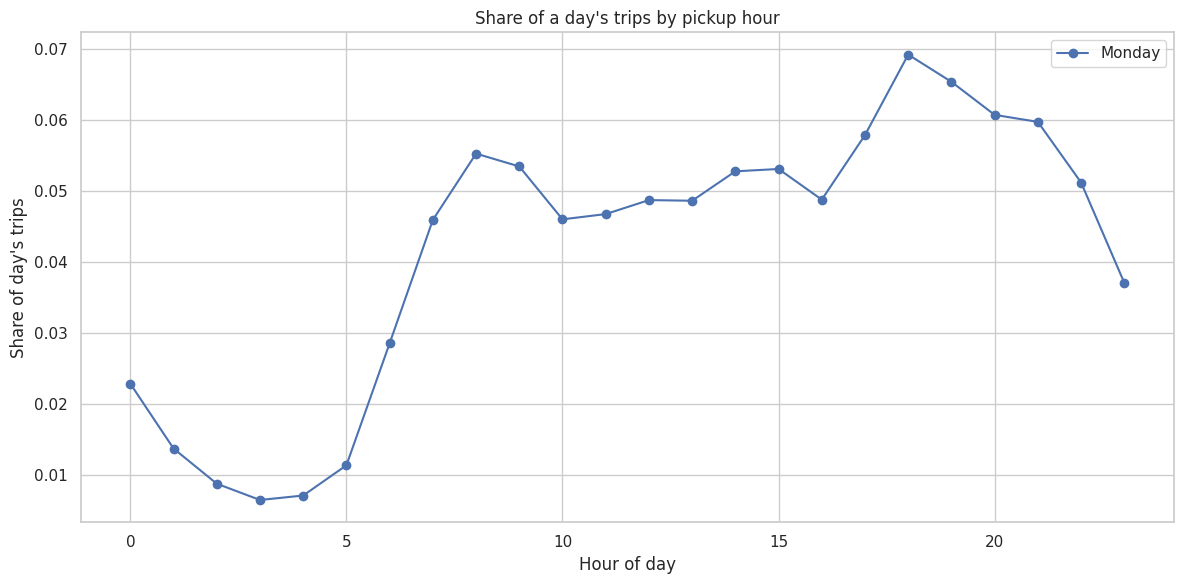
\includegraphics[width=\linewidth]{q3_2_profiles.png}
  \caption{Normalised per-day hourly profile.}
\end{subfigure}

\end{figure}

\textbf{Observations and possible explanations.}
\begin{itemize}
  \item \textbf{Monday--Wednesday} peak at \textbf{18:00--19:00} --- the
        classic end-of-work commute, when taxis are used for the
        door-to-door trip home and for after-work socialising.
  \item \textbf{Thursday and Friday} shift slightly later
        (\textbf{21:00} and \textbf{19:00}) and grow in peak volume:
        as the week ends, after-work demand merges into evening
        and nightlife demand.
  \item \textbf{Saturday} peaks at \textbf{23:00}, and \textbf{Sunday}
        peaks at \textbf{00:00}. The weekend peak is late-night
        demand (bars, restaurants, clubs) that spills past midnight.
  \item The weekday \emph{morning} peak at 08:00 is visible in the
        heatmap but is consistently smaller than the evening peak;
        this is consistent with many commuters using the subway in
        the morning and taking taxis in the evening.
  \item Sunday is the only day whose demand trough is the early
        morning and whose afternoon is comparatively strong
        (brunch, shopping, returns from weekend trips).
\end{itemize}

\subsection{Q3.3 --- Weekdays versus weekends}
The weekday peak hour is \textbf{19:00 (512 trips/day on average)}; the
weekend peak hour is \textbf{00:00 (457 trips/day)}. The full hourly
curves are shown in Figure 3.

\begin{figure}[H]
\centering
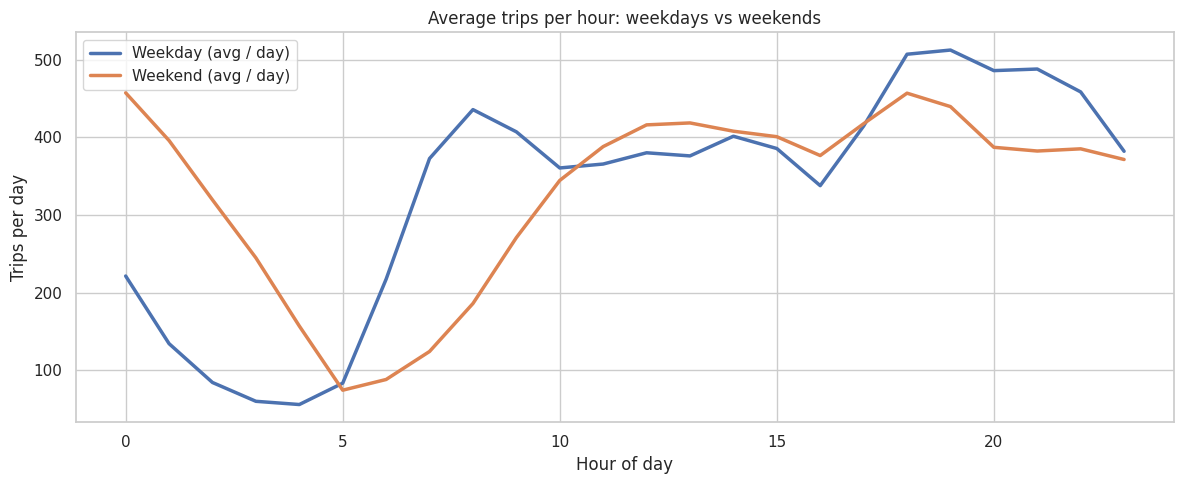
\includegraphics[width=0.92\textwidth]{q3_3_weekday_vs_weekend.png}
\caption{Average trips per hour: weekdays versus weekends.}
\end{figure}

\textbf{Differences and explanations.}
\begin{itemize}
  \item \textbf{Weekdays} show the two-peak structure: a small
        morning peak around 08:00 and a large evening peak around
        18:00--19:00. This is the commuting signature: demand is
        structured by fixed work schedules.
  \item \textbf{Weekends} have \emph{no} morning peak. Demand grows
        through the afternoon and peaks at midnight (Saturday night
        into Sunday). Weekend demand is structured by leisure
        schedules: dinner, nightlife, tourism, shopping.
  \item The \textbf{crossover} in the small hours of Saturday and
        Sunday is the largest structural difference in the week:
        weekday 03:00--04:00 is the daily minimum, whereas weekend
        03:00--04:00 remains high because nightlife demand is still
        active.
\end{itemize}

 \newpage
\subsection{Q3.4 --- Major holidays}
The correct 2016 dates are: \textbf{Martin Luther King Day, Monday
18 January}; \textbf{Valentine's Day, Sunday 14 February};
\textbf{St.\ Patrick's Day, Thursday 17 March}; \textbf{Easter Sunday,
27 March}; and \textbf{Memorial Day, Monday 30 May}. Each holiday is
compared to the average of the same weekday across the rest of the
period so that the day-of-week effect is removed. Figure 4 shows the hourly profiles.

\begin{figure}[H]
\centering
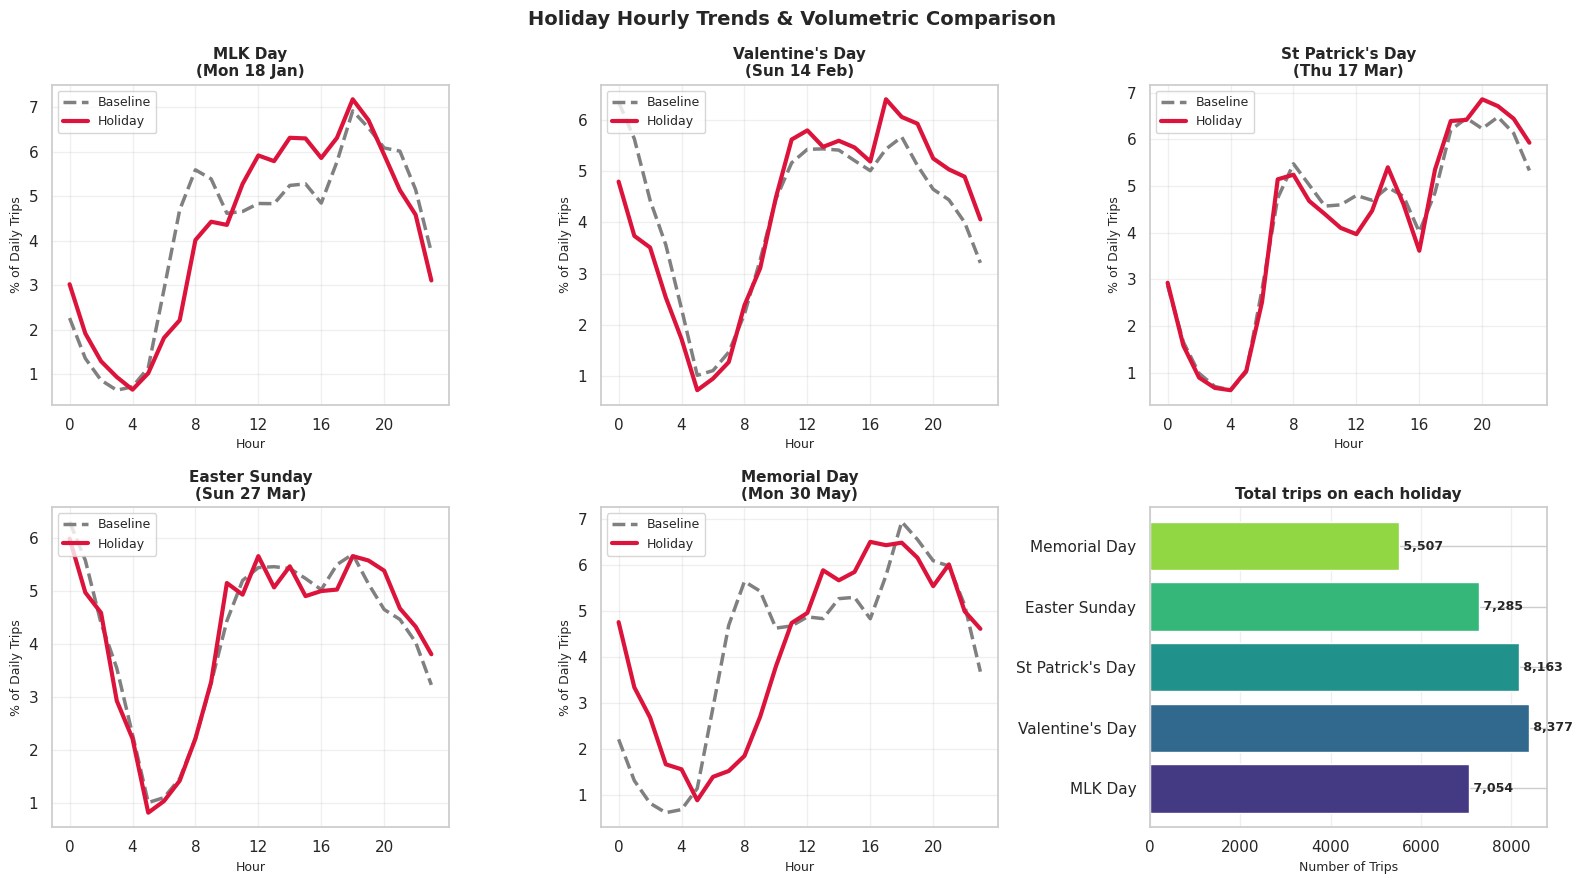
\includegraphics[width=0.96\textwidth]{q3_4_holidays.png}
\caption{Hourly demand on each major 2016 holiday versus the
same-weekday baseline.}
\end{figure}

\begin{table}[H]
\centering
\caption{Summary of holiday effects relative to the same weekday.}
\begin{tabular}{p{3.4cm}p{4.7cm}p{7.0cm}}
\toprule
\textbf{Holiday} & \textbf{Pattern vs.\ baseline} & \textbf{Interpretation} \\
\midrule
MLK Day (Mon 18 Jan) &
  Morning commute peak vanishes; total volume 15--25\,\% lower;
  demand shifts to the afternoon. &
  Public holiday: no commute, reduced business travel. \\
Valentine's Day (Sun 14 Feb) &
  Evening demand (18:00--22:00) higher than a normal Sunday;
  afternoon similar; morning unchanged. &
  Restaurant/date-night demand. \\
St.\ Patrick's Day (Thu 17 Mar) &
  Evening and late-night demand (18:00--02:00) sharply elevated;
  usual 18:00 commute absorbed into a much larger nightlife peak. &
  Pub culture and parade aftermath. \\
Easter Sunday (Sun 27 Mar) &
  Total volume 20--30\,\% lower; morning and midday unusually
  quiet; modest afternoon bump. &
  Family day at home; many businesses closed. \\
Memorial Day (Mon 30 May) &
  Morning commute peak vanishes; afternoon/early-evening demand
  slightly higher than a normal Monday; total volume similar
  to a normal Monday. &
  Long-weekend leisure travel (beaches, BBQs, airports) offsets
  the loss of business travel. \\
\bottomrule
\end{tabular}
\end{table}

Holidays change \emph{the shape} of the day more than
\emph{the total}. On every public holiday the weekday morning commute peak disappears; the evening/late-night peak then moves according to the cultural nature of the holiday (Valentine's and St.\ Patrick's = evening
spikes; Easter = quiet; Memorial Day = leisure afternoon).


\newpage

\subsection{Q3.5 --- Average speed by hour of day}

\begin{table}[H]
\centering
\caption{Mean and median speed (km/h) by pickup hour.}

\begin{tabular}{rrr|rrr}
\toprule
\textbf{Hour} & \textbf{Mean} & \textbf{Median} &
\textbf{Hour} & \textbf{Mean} & \textbf{Median} \\
\midrule
0  & 17.76 & 16.09 & 12 & 12.30 & 10.81 \\
1  & 18.53 & 17.03 & 13 & 12.49 & 11.07 \\
2  & 18.96 & 17.60 & 14 & 12.27 & 10.93 \\
3  & 20.04 & 18.58 & 15 & 12.14 & 10.96 \\
4  & 22.31 & 20.63 & 16 & 12.62 & 11.52 \\
\textbf{5}  & \textbf{24.57} & \textbf{22.83} & 17 & 12.55 & 11.53 \\
6  & 20.61 & 19.03 & 18 & 12.59 & 11.47 \\
7  & 15.85 & 14.34 & 19 & 13.65 & 12.28 \\
8  & 13.04 & 11.44 & 20 & 15.20 & 13.71 \\
9  & 12.68 & 11.00 & 21 & 15.85 & 14.34 \\
10 & 12.83 & 11.22 & 22 & 16.08 & 14.60 \\
11 & 12.48 & 10.97 & 23 & 16.95 & 15.30 \\
\bottomrule
\end{tabular}
\end{table}

\begin{figure}[H]
\centering
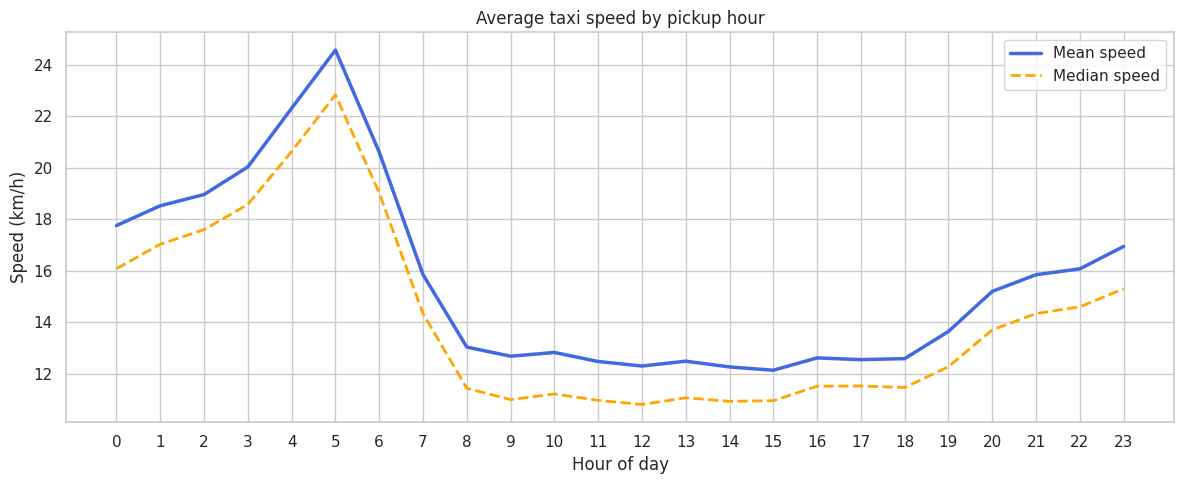
\includegraphics[width=0.92\textwidth]{q3_5_speed_by_hour.png}
\caption{Mean and median taxi speed by pickup hour.}

\end{figure}

\textbf{Findings.}
\begin{itemize}
  \item \textbf{Fastest hour: 05:00, mean 24.57\,km/h
        (median 22.83\,km/h).} Empty roads, green lights and airport
        runs via the Van Wyck / Belt Parkway dominate before the
        morning rush. Hours 04:00--06:00 are consistently the fastest
        block of the day.
  \item \textbf{Slowest hour: 15:00, mean 12.14\,km/h
        (median 10.96\,km/h).} The morning rush (08:00--10:00) is
        similar: mean 12.7--13.0\,km/h, i.e.\ roughly half the
        early-morning speed. The evening rush (17:00--19:00) is only
        slightly faster, with the 19:00 mean rising to
        13.65\,km/h as the rush thins.
  \item \textbf{Interpretation.} The speed curve is essentially the
        inverse of the demand curve: the two hours of highest demand
        are also the two hours of lowest speed. This is the central
        operational tension of the taxi business, and it is why the
        peak-hour demand in Q3.2 is so visible in the data---the same
        trips take much longer, so more cars are on the road at once.
\end{itemize}

% =====================================================================
\section{Conclusion}
% =====================================================================
Data cleaning removed 1.58\,\% of rows using six physically motivated
filters, producing a bounded and realistic working dataset of
1{,}442{,}031 trips. Feature generation added haversine distance,
average speed, and the day/hour/weekend features required for the
time-based analysis. The time-based analysis shows that (i) Friday is
the busiest day and Monday the quietest; (ii) each day has a
characteristic peak hour, with weekdays peaking in the evening commute
and weekends peaking near midnight; (iii) weekends differ from weekdays
by losing the morning commute peak and gaining a late-night plateau;
(iv) the five major 2016 holidays reshape the daily demand profile
rather than merely reducing it; and (v) mean speed is lowest during the
morning and evening rush (12.1--13.0\,km/h) and highest between 04:00
and 06:00 (up to 24.6\,km/h), exactly inverting the demand curve.

\end{document}